\def\mySecNum{11.2}
\mySection{\mySecNum~Understanding risk-neutral pricing}
%-------------- start slide -------------------------------%{{{ 1
\begin{frame}[fragile,t]
	\frametitle{Risk-Neutral Probability}
	\begin{center}

		Recall the binomial option pricing formula:

		\begin{align*}
			C = \Delta S + B = e^{-rh} \bigg[ p^* C_u + (1-p^*) C_d\bigg]
		\end{align*}

		\begin{align*}
			p^* = \frac{e^{(r-\delta)h}-d}{u-d} \quad  \sim \quad  \parbox{12em}{\textcolor{magenta}{risk-neutral probability}\\ that the stock will go up}
		\end{align*}
		\bigskip
		\mySeparateLine
		\bigskip
		\begin{align*}
			p^* = \frac{e^{(r-\delta)h}-d}{u-d} \quad  \Longleftrightarrow \quad p^* uS e^{\delta h} + (1-p^*) dS e^{\delta h} = e^{rh} S
		\end{align*}
	\end{center}
\end{frame}
%-------------- end slide -------------------------------%}}}
%-------------- start slide -------------------------------%{{{ 1
\begin{frame}[fragile,t]
	\begin{center}
		\begin{minipage}{0.7\textwidth}
			\centering

			Two offers:
			\begin{enumerate}
				\item[(a)] \$1000 cash
				\item[(b)] \$2000 or \$0 cash with probability $1/2$ for each
					\bigskip
				\item[] Both offers have the same expected return,
				\item[] while (b) bears risk and (a) does not.
			\end{enumerate}
		\end{minipage}
	\end{center}
	\pause
	\vfill

	A \textcolor{cyan}{risk-averse investor} prefers (a).

	\vfill

	A \textcolor{magenta}{risk-neutral investor} is indifferent between a sure thing and a risky bet with an expected payoff equal to the value of the sure thing.
	Hence, he/she prefers equally to (a) and (b).
\end{frame}
%-------------- end slide -------------------------------%}}}
%-------------- start slide -------------------------------%{{{ 1
\begin{frame}[fragile]
\begin{center}

	The option pricing formula can be said to price options \\
	\textcolor{magenta}{as if investors are risk-neutral}
	\bigskip

	Note that we are not assuming that investors are actually risk-neutral, and that risky assets are actually expected to earn the risk-free rate of return.
\end{center}
\end{frame}
%-------------- end slide -------------------------------%}}}
%-------------- start slide -------------------------------%{{{ 1
\begin{frame}[fragile,t]
	\frametitle{Pricing an option using real probability}
\begin{itemize}
	\item Suppose that the continuously compounded expected return on the stock is $\alpha$ and that the stock does not pay dividends.
	\item If $p$ is the true probability of the stock going up, $p$ must be consistent with $u$, $d$ and $\alpha$
		\begin{align*}
			puS + (1-p) dS = e^{\alpha h} S
		\end{align*}
	\item Solving for $p$ gives us
		\begin{align*}
			p= \frac{e^{\alpha h}-d}{u-d}
		\end{align*}
	\item For $p$ to be a probability, we have to have  $u\ge e^{\alpha h}\ge d$.
	\item Using this $p$, the actual expected payoff to the option one period is
		\begin{equation*}
			p C_u + (1-p) C_d = \frac{e^{\alpha h}-d}{u-d} C_u + \frac{u-e^{\alpha h}}{u-d}C_d.
		\end{equation*}
\end{itemize}
\end{frame}
%-------------- end slide -------------------------------%}}}
%-------------- start slide -------------------------------%{{{ 1
\begin{frame}[fragile,t]
		\begin{center}
	    At what rate do we discount this expected payoff?
			\begin{equation*}
				p C_u + (1-p) C_d = \frac{e^{\alpha h}-d}{u-d} C_u + \frac{u-e^{\alpha h}}{u-d}C_d
			\end{equation*}
			\mySeparateLine
			\bigskip
			\pause

	    It is not correct to discount the option at the expected return on the stock, $\alpha$, because the option is equivalent to a leveraged investment in the stock and hence is riskier than the stock
		\end{center}
\end{frame}
%-------------- end slide -------------------------------%}}}
%-------------- start slide -------------------------------%{{{ 1
\begin{frame}[fragile,t]
		\begin{center}
	    At what rate do we discount this expected payoff?
			\begin{equation*}
				p C_u + (1-p) C_d = \frac{e^{\alpha h}-d}{u-d} C_u + \frac{u-e^{\alpha h}}{u-d}C_d
			\end{equation*}
			\mySeparateLine
			\bigskip
			\pause


			\begin{itemize}
				\item Denote the appropriate per-period discount rate for the option as $\gamma$
				\item Since an option is equivalent to holding a portfolio consisting of $\Delta$ shares of stock and $B$ bonds, the expected return on this portfolio is
					\begin{equation*}
						e^{\gamma h} = \frac{S \Delta}{S \Delta +B} e^{\alpha h} + \frac{B}{S\Delta +B}e^{r h}
					\end{equation*}
				\item Hence, the discounted at this appropriate discount rate, the price for the option
					should be
					\begin{equation*}
						C = e^{-\gamma h} \left[ \frac{e^{\alpha h}-d}{u-d}C_u+ \frac{u- e^{\alpha h}}{u-d}C_d\right]
					\end{equation*}
				\item By setting $\alpha=r$, one obtains the simplest pricing procedure.
				\item This gives an alternative way to compute the option price, instead of $\Delta S+B$.
			\end{itemize}
		\end{center}
\end{frame}
%-------------- end slide -------------------------------%}}}
%-------------- start slide -------------------------------%{{{ 1
\begin{frame}[fragile,t]
	\begin{center}
		One can use either
		\bigskip
		\begin{equation*}
			\textcolor{magenta}{C= \Delta S + B}
		\end{equation*}

		\bigskip
		or
		\bigskip

		\begin{equation*}
			\textcolor{cyan}{C = e^{-\gamma h} \left[ \frac{e^{\alpha h}-d}{u-d}C_u+ \frac{u- e^{\alpha h}}{u-d}C_d\right]}
		\end{equation*}
		\bigskip

		to compute the option price
	\end{center}
	\pause
	\mySeparateLine
	\begin{itemize}
		\item \textcolor{magenta}{First equation} is more efficient
		\item For the \textcolor{cyan}{second one}, in order to compute $\gamma$, one needs to computer  $\Delta$ and  $B$
			first and then obtains $\gamma$ via
			\begin{equation*}
					e^{\gamma h} = \frac{S \Delta}{S \Delta +B} e^{\alpha h} + \frac{B}{S\Delta +B}e^{r h}
			\end{equation*}
	\end{itemize}
\end{frame}
%-------------- end slide -------------------------------%}}}
%-------------- start slide -------------------------------%{{{ 1
\begin{frame}[fragile,t]
\begin{enumerate}
	\item[] Given the continuously compounded expected return of the stock $\alpha$
		\bigskip
	\item Compute the probability that stock goes up
		\begin{align*}
			p=\frac{e^{\alpha h}-d}{u-d}
		\end{align*}
	\item Compute the actual expected payoff (to be discounted)
		\begin{align*}
			X := p C_u + (1-p) C_d
		\end{align*}
	\item Using $r$ and $\delta$ to compute  $\Delta$ and $B$:
		\begin{align*}
			\Delta = e^{-\delta h}\frac{C_u-C_d}{S(u-d)} \qquad \text{and} \qquad
			B=e^{-rh}\frac{uC_d-dC_u}{u-d}.
		\end{align*}
	\item Compute the discounted rate $\gamma$:
		\begin{align*}
			\gamma = \frac{1}{h}\log\left(\frac{S\Delta}{S\Delta+B}e^{\alpha h} + \frac{B}{S\Delta+B}e^{r h}\right)
		\end{align*}
	\item Finally, the option price should be the discounted value:
		\begin{align*}
			X e^{-\gamma h}.
		\end{align*}
\end{enumerate}
\end{frame}
%-------------- end slide -------------------------------%}}}
%-------------- start slide -------------------------------%{{{ 1
\begin{frame}[fragile,t]
		% \textcolor{gray}{Interested students should check out two examples on p. 328 -- 330 using the second formula.}
	\frametitle{An one-period example}
	\begin{center}
		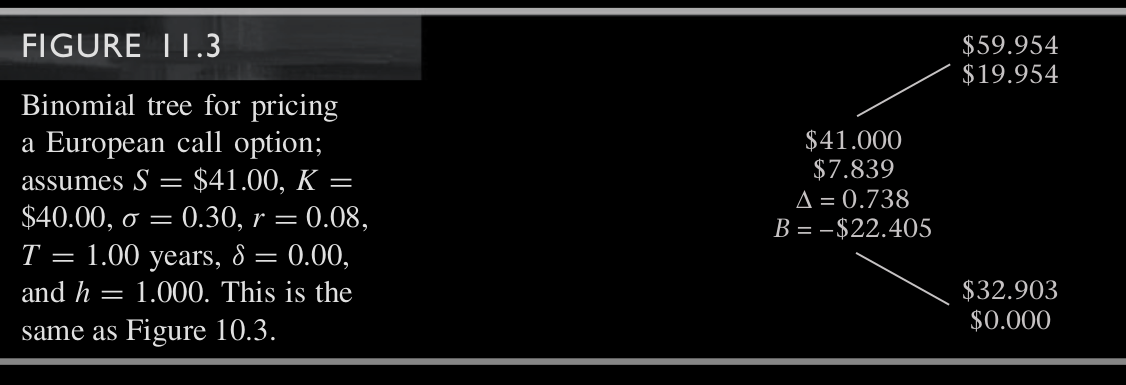
\includegraphics[scale=0.25]{figs/Figure-11-3.png}
	\end{center}
\end{frame}
%-------------- end slide -------------------------------%}}}
%-------------- start slide -------------------------------%{{{ 1
\begin{frame}[fragile,t]
		% \textcolor{gray}{Interested students should check out two examples on p. 328 -- 330 using the second formula.}
	\frametitle{A multi-period example}
	\begin{center}
		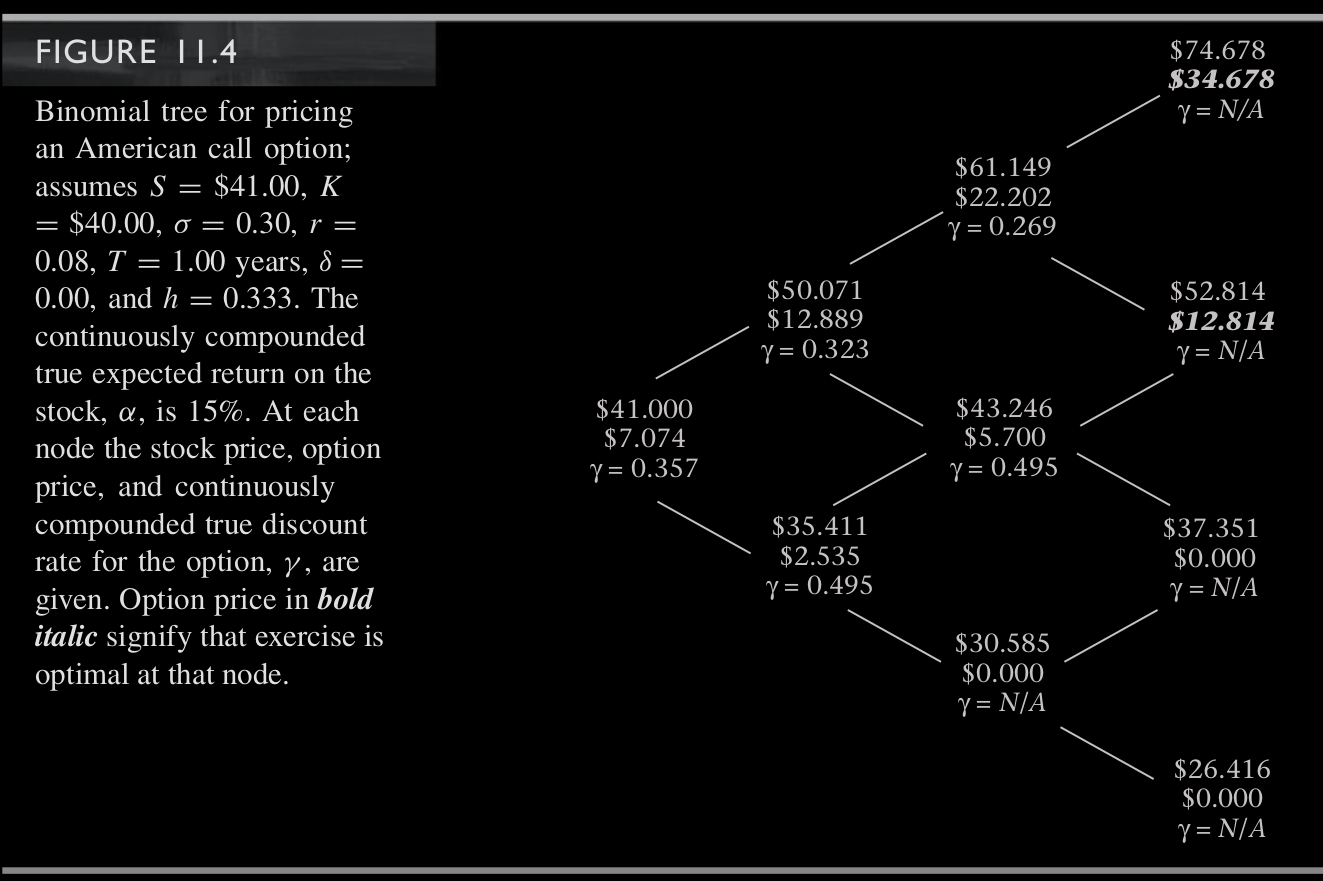
\includegraphics[scale=0.25]{figs/Figure-11-4.png}
	\end{center}
\end{frame}
%-------------- end slide -------------------------------%}}}
